
\vspace{-8mm}
\section{Introduction}
Large Language Models (LLMs) have shown impressive performance across multiple disciplines, including conversational AI and language translation.
However, pre-training and fine-tuning LLMs require not only a huge amount of computation but is also memory intensive. The memory requirements include not only billions of trainable parameters,  but also their gradients and optimizer states (e.g., gradient momentum and variance in Adam) that can be larger than parameter storage themselves  ~\citep{raffelExploringLimitsTransfer2020,touvronLlamaOpenFoundation2023,chowdheryPaLMScalingLanguage2022}. For example, pre-training a LLaMA 7B model from scratch with a single batch size requires at least 58 GB memory (14GB for trainable parameters, 42GB for Adam optimizer states and weight gradients, and 2GB for activations\protect\footnotemark[1]).
This makes the training not feasible on consumer-level GPUs such as NVIDIA RTX 4090 with 24GB memory.





\definecolor{cus_color}{rgb}{22, 96, 55}


\makeatletter
\newcommand{\removelatexerror}{\let\@latex@error\@gobble}
\makeatother


\begin{figure}[!t]
\centering
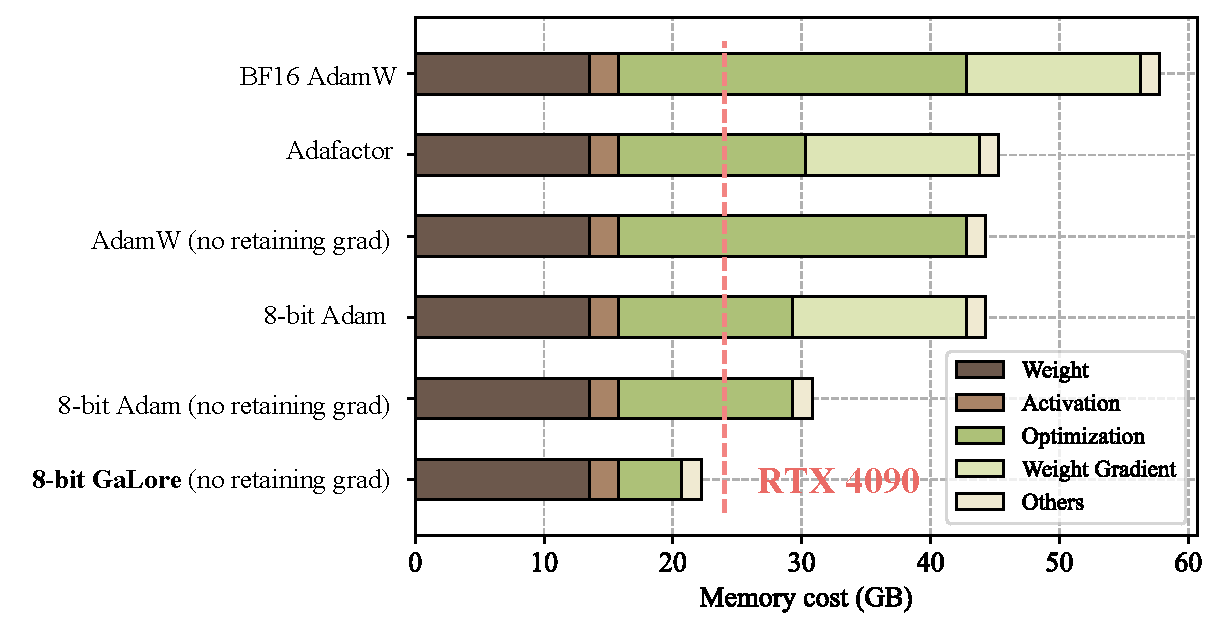
\includegraphics[width=1\columnwidth]{figures/files/memory_breakdown.pdf}
\vskip -0.11in
\caption{\small{Estimated memory consumption of pre-training a LLaMA 7B model with a token batch size of 256 on a single device, without activation checkpointing and memory offloading\protect\footnotemark[2]. Details refer to Section~\ref{sec:memory_measure}.}}
\label{fig:memory_breakdown} 
\vskip -0.15in
\end{figure}
\footnotetext[1]{The calculation is based on LLaMA architecture, BF16 numerical format, and maximum sequence length of 2048.}
\footnotetext[2]{In the figure, ``no retaining grad'' denotes the application of per-layer weight update to reduce memory consumption of storing weight gradient \citep{lvFullParameterFinetuning2023}.}
\SetAlFnt{\fontsize{8pt}{9pt}\selectfont}
\SetAlCapFnt{\fontsize{8pt}{9pt}\selectfont}
\begin{algorithm}[t]
    \SetAlgoLined
        \PyCode{for weight in model.parameters():} \\
        \Indp   %
            \PyCode{grad = weight.grad} \\ 
            \PyComment{original space -> compact space} \\
            \PyCode{lor\_grad = \textbf{project}(grad)} \\
            \PyComment{update by Adam, Adafactor, etc.} \\
            \PyCode{lor\_update = \textbf{update}(lor\_grad)} \\
            \PyComment{compact space -> original space} \\
            \PyCode{update = \textbf{project\_back}(lor\_update)} \\
            \PyCode{weight.data += update} \\
        \Indm %
    \caption{\fontsize{8pt}{9pt}\selectfont{\lowrank{}, PyTorch-like}}
    \label{alg:code_box}
\end{algorithm}


In addition to engineering and system efforts, such as gradient checkpointing~\cite{chenTrainingDeepNets2016}, memory offloading~\cite{rajbhandariZeROMemoryOptimizations2020}, etc., to achieve faster and more efficient distributed training, researchers also seek to develop various optimization techniques to reduce the memory usage during pre-training and fine-tuning. 

\def\rr{\mathbb{R}}

Parameter-efficient fine-tuning (PEFT) techniques allow for the efficient adaptation of pre-trained language models (PLMs) to different downstream applications without the need to fine-tune all of the model's parameters \citep{dingDeltaTuningComprehensive2022}.
Among them, the popular Low-Rank Adaptation (LoRA~\citet{huLoRALowRankAdaptation2021}) \emph{reparameterizes} weight matrix $W\in \rr^{m\times n}$ into $W = W_0 + BA$, where $W_0$ is a frozen full-rank matrix and $B\in\rr^{m\times r}$, $A\in\rr^{r\times n}$ are additive low-rank adaptors to be learned. Since the rank $r \ll \min(m,n)$, $A$ and $B$ contain fewer number of trainable parameters and thus smaller optimizer states. LoRA has been used extensively to reduce memory usage for fine-tuning in which $W_0$ is the frozen pre-trained weight. Its variant ReLoRA is also used in pre-training, by periodically updating $W_0$ using previously learned low-rank adaptors \citep{lialinReLoRAHighRankTraining2023}.

However, many recent works demonstrate the limitation of such a low-rank reparameterization. For fine-tuning, LoRA is not shown to reach a comparable performance as full-rank fine-tuning~\cite{xiaChainLoRAEfficient2024}.
For pre-training from scratch, it is shown to require a full-rank model training as a warmup \citep{lialinReLoRAHighRankTraining2023}, before optimizing in the low-rank subspace. There are two possible reasons: (1) the optimal weight matrices may not be low-rank, and (2) the reparameterization changes the gradient training dynamics.

{\bf Our approach: }To address the above challenge, we propose Gradient Low-Rank Projection (\textbf{\lowrank}), a training strategy that allows \emph{full-parameter} learning but is more \emph{memory-efficient} than common low-rank adaptation methods, such as LoRA. Our key idea is to leverage the slow-changing low-rank structure of the \emph{gradient} $G\in\rr^{m\times n}$ of the weight matrix $W$, rather than trying to approximate the weight matrix itself as low rank. 

We first show theoretically that the gradient matrix $G$ becomes low-rank during training. Then, we propose \lowrank{} that computes two projection matrices $P\in \rr^{m\times r}$ and $Q\in \rr^{n\times r}$ to project the gradient matrix $G$ into a low-rank form $P^\top G Q$.
In this case, the memory cost of optimizer states, which rely on component-wise gradient statistics, can be substantially reduced. Occasional updates of $P$ and $Q$ (e.g., every 200 iterations) incur minimal amortized additional computational cost.
\lowrank is more memory-efficient than LoRA as shown in Table~\ref{tab:lora_compare}.
In practice, this yields up to 30\% memory reduction compared to LoRA during pre-training.




We demonstrate that \lowrank{} works well in both LLM pre-training and fine-tuning. When pre-training LLaMA 7B on C4 dataset, 8-bit \lowrank, combined with 8-bit optimizers and layer-wise weight updates techniques, achieves comparable performance to its full-rank counterpart, with less than 10\% memory cost of optimizer states. 

Notably, for pre-training, \lowrank{} keeps low memory throughout the entire training, without requiring full-rank training warmup like ReLoRA.  
Thanks to \lowrank's memory efficiency, it is possible to train LLaMA 7B from scratch on a single GPU with 24GB memory (e.g., on NVIDIA RTX 4090), without any costly memory offloading techniques (Fig.~\ref{fig:memory_breakdown}).

\lowrank{} is also used to fine-tune pre-trained LLMs on GLUE benchmarks with comparable or better results than existing low-rank methods. 
When fine-tuning RoBERTa-Base on GLUE tasks with a rank of 4, \lowrank{} achieves an average score of 85.89, outperforming LoRA, which achieves a score of 85.61.

As a gradient projection method, \lowrank{} is independent of the choice of optimizers and can be easily plugged into existing ones with only two lines of code, as shown in Algorithm~\ref{alg:code_box}. Our experiment (Fig.~\ref{fig:compare_optimizer}) shows that it works for popular optimizers such as AdamW, 8-bit Adam, and Adafactor. In addition, its performance is insensitive to very few hyper-parameters it introduces. We also provide theoretical justification on the low-rankness of gradient update, as well as the convergence analysis of \lowrank. 






















